\chapter{Installation and Setup}
\label{chap:installation}

\ChapterMeta{
This chapter guides you through establishing a functional \yolozu{} environment and validating it via preliminary sanity checks.
}{
It ensures the creation of a reproducible toolchain while explicitly detailing backend availability and dependencies.
}{
Python 3.10 or newer is mandatory. Optional extras vary based on the selected backend; notably, TensorRT workflows typically necessitate a Linux environment equipped with an NVIDIA GPU.
}
\ChapterAudience{Read this chapter when you are setting up a fresh environment or checking which extras and runtimes you actually need.}


\section{Python Requirements}
\yolozu{} targets Python 3.10 and newer.
The candidate-wheel sample workflow checks Python 3.10--3.14 on Linux,
Python 3.14 on macOS, and Python 3.12 on Windows. One Linux/Python 3.10 lane
uses the declared core and COCO dependency floors. These are configured checks;
read each run's report for the versions and outcomes actually observed.
Wheel hashes distinguish a local candidate from published code with the same
version string. See \path{docs/versions.md}; this matrix does not qualify GPU
inference or external training runtimes.

\section{Pip Installation (User Path)}
\subsection{First successful run from the installed package}
On macOS/Linux, run these commands in a writable directory. A virtual environment
keeps this installation separate from system-managed Python. No source checkout
or model download is needed for this CPU-only path:
\begin{lstlisting}[language=bash]
python3 -m venv .venv
source .venv/bin/activate
python3 -m pip install yolozu
yolozu doctor --proof \
  --output reports/first_run/doctor.json \
  --proof-dir reports/first_run/proof
yolozu demo instance-seg --background synthetic --inference none \
  --run-dir reports/first_run/demo
\end{lstlisting}
For Windows PowerShell commands, see \path{docs/install.md}. If \cmd{yolozu}
is not found, use \cmd{python3 -m yolozu} from the same environment.

The doctor proof writes \path{proof_report.json}, \path{eval_report.json}, and
\path{known_predictions.json} under \path{reports/first_run/proof}. Check
\cmd{status=pass} in the proof report. The demo writes a report and PNG overlays under
\path{reports/first_run/demo}.

These are deterministic installation and evaluation checks. They use known or
synthetic predictions, so their scores and overlays do not measure trained-model
accuracy. Use your own predictions and dataset for that next step:
\begin{lstlisting}[language=bash]
yolozu validate predictions /path/to/predictions.json --strict
yolozu eval-coco --help
\end{lstlisting}
Replace the placeholder with your artifact path. Chapter~\ref{chap:evaluation-workflows}
explains evaluation; \path{docs/cpu_only_dod.md} gives the full proof-based sequence.
Use \cmd{yolozu --help} to explore commands or \cmd{yolozu guide --goal first-run}
for guided next steps.

\subsection{Reusable labeled sample}
The command below, available from version 4.8.0, creates eight synthetic images with YOLO
bounding-box labels, two classes, and a deliberately empty validation image.
In a virtual environment, install the package with the COCO extra before evaluating:
\begin{lstlisting}[language=bash]
python3 -m pip install 'yolozu[coco]==4.8.0'
python3 -m yolozu demo dataset --run-dir reports/labeled_sample --seed 0
python3 -m yolozu validate dataset reports/labeled_sample --split val --strict
python3 -m yolozu validate predictions \
  reports/labeled_sample/predictions.json --strict
python3 -m yolozu eval-coco --dataset reports/labeled_sample --split val \
  --predictions reports/labeled_sample/predictions.json \
  --output reports/labeled_sample_coco.json
\end{lstlisting}
Open \path{labeled_preview.png} in the generated directory to inspect the labels.
Copy the entire directory to reuse it: paths are relative, and the manifest
records the seed, recipe, package versions, and file hashes. Existing output
paths are refused. The known predictions come from the labels, so an AP near
1.0 checks the workflow, not model accuracy. Replace them with model outputs
before interpreting accuracy on your own data. See \path{docs/labeled_sample.md}
for the layout and external-tool path caveat.

\paragraph{Stable versus qualified paths.}
The default stable path is CPU-first install plus predictions evaluation.
macOS/MPS is a \textbf{qualification path}.
\cmd{torch.backends.mps.is_available()} reports whether this process can use MPS.
A true result does not qualify every model, operator, precision, or workload.

The doctor report includes a validated \cmd{environment_profile}.
Its bounded probes omit host identifiers and keep failed or unsupported facts
unknown. This EnvironmentProfile interface contract records the observed
configuration; it is not model qualification evidence and does not make an
Experimental adaptive pipeline available.

\subsection{Optional adaptive interfaces}
This subsection is for callers integrating adaptive image pipelines. It is not
needed for the first-run or predictions-evaluation path above.

The installed package also contains three non-promoted adaptive Candidate bundle
records matching the existing model zoo. Their weight metadata is pinned, but their
execution binding is unbound. The bounded loader validates this registry and lifecycle
SSOT without importing a model runtime or downloading assets. A caller-supplied workspace catalog remains
\cmd{operator\_asserted} and nonselectable; registry integrity alone is not
qualification evidence. A non-executing candidate-screening provider is packaged,
and the repository-managed stream currently contains two \cmd{hold} records.
Workspace screening input remains
\cmd{operator\_asserted}, and a pass record alone cannot register or execute a
bundle. The Experimental \cmd{yolozu qualify-image-pipeline}
command is installed, but the unbound Candidate records and empty runner map make the default
invocation fail actionably without dummy evidence. Its \cmd{--help} documents
the exact-bundle, timeout, pinned-input, and managed-output interface contract.

The Experimental \cmd{yolozu update-image-pipeline-lifecycle} command is also
installed. It defaults to a no-write dry-run and requires an approved public review,
exact observed heads, and \cmd{--approve} before appending one lifecycle event.
Its rollback operation can restore only the complete historical profile set to a
previously assigned, currently eligible same-family target or explicit \cmd{none}.
The event records the exact historical target-assignment digest.
It does not provide automatic
rollback or make the Candidate records executable. No lifecycle event is added by
installing this interface contract.

The installed Python API also exposes \cmd{ManagedOutputTransaction} for
repository-owned qualification and processing outputs. It uses bounded manifests,
directory-relative no-follow mutation, and fail-closed recovery on POSIX. It does
not make a model adapter or runnable model bundle available. The installed
recommendation, selector, and pinned-processing interface contracts are verified,
but the Candidate-only registry, held screenings, empty public evidence stream, and empty runner maps
make the default recommendation abstain with \cmd{maturity\_disallowed} and processing
reject with \cmd{selection\_required}.
Positive selector and executor tests use internal fixtures rather than public
qualification evidence. The managed output path does not silently weaken its guarantee
on platforms without the required primitives. Atomic visibility is scoped to a
successful same-filesystem rename probe; power-loss durability remains best-effort.

\subsection{First-failure checklist}
If the first run fails, do not jump straight into backend debugging. Check the
artifact path first, then the optional runtime that produced it. The checklist
below gives a symptom, likely cause, and verification command for the common
first-run failures; the Troubleshooting chapter expands the same cases into a fuller
troubleshooting playbook.

\begin{description}
  \item[Symptom: \cmd{pip install yolozu} fails.] Likely cause: Python or the
  packaging toolchain is too old. Verification command:
\begin{lstlisting}[language=bash]
python3 --version
python3 -m pip --version
\end{lstlisting}

  \item[Symptom: missing import after install.] Likely cause: the workflow needs
  an optional extra. Verification command:
\begin{lstlisting}[language=bash]
python3 -m pip install 'yolozu[demo]'
python3 -m pip install 'yolozu[onnxrt]'
\end{lstlisting}

  \item[Symptom: COCO metrics look shifted.] Likely cause: \cmd{category_id}
  values do not match the evaluator class mapping. Verification command:
\begin{lstlisting}[language=bash]
yolozu validate predictions <predictions.json> --strict
\end{lstlisting}

  \item[Symptom: predictions schema error.] Likely cause: required fields,
  paths, or task-specific payloads are missing. Verification command:
\begin{lstlisting}[language=bash]
yolozu validate predictions <predictions.json> --strict
\end{lstlisting}

  \item[Symptom: ONNX Runtime model-load error.] Likely cause: ORT cannot load
  the exported ONNX IR/opset or runtime build. Verification command:
\begin{lstlisting}[language=bash]
python3 -c "import onnxruntime as ort; print(ort.__version__)"
\end{lstlisting}

  \item[Symptom: TensorRT command fails locally.] Likely cause: TensorRT needs a
  compatible Linux/NVIDIA/CUDA stack. In a source checkout, inspect the preflight options:
\begin{lstlisting}[language=bash]
python3 tools/gpu_validation_preflight.py --help
\end{lstlisting}

  \item[Symptom: metrics changed after protocol edit.] Likely cause: evaluation
  thresholds, class order, score filtering, NMS, or protocol pins changed.
  Verification command:
\begin{lstlisting}[language=bash]
yolozu eval-coco --help
\end{lstlisting}
  Then inspect the saved evaluation report and the protocol used by both runs.
\end{description}

Optional extras let you install only the dependencies you need for a given workflow:
\begin{lstlisting}[language=bash]
python3 -m pip install 'yolozu[demo]'    # PyTorch demonstration utilities (includes timm + opencv-contrib + transformers for depth demo)
python3 -m pip install 'yolozu[onnxrt]'  # ONNX Runtime tooling
python3 -m pip install 'yolozu[coco]'    # COCOeval support
python3 -m pip install 'yolozu[full]'    # Comprehensive installation
\end{lstlisting}

If you are operating from a source checkout (editable install), extras use the dot-prefix form:
\begin{lstlisting}[language=bash]
python3 -m pip install -e '.[demo]'
\end{lstlisting}

\subsection{Optional demos (CPU)}
The demo commands are intentionally designed to keep the invocation short:
\begin{lstlisting}[language=bash]
python3 -m pip install -U 'yolozu[demo]'
yolozu demo
yolozu demo instance-seg
yolozu demo instance-seg-tta
yolozu demo instance-seg --background yolo-bbox --yolo-root data/smoke --yolo-split val --inference none
yolozu demo keypoints
yolozu demo pose
yolozu demo pose --backend aruco  # cached sample in demo_output/pose/_samples
yolozu demo pose --backend densefusion
yolozu demo depth
yolozu demo depth --compare
yolozu demo train  # downloads ResNet18 on first run
yolozu demo continual --compare --markdown
\end{lstlisting}

\noindent Note: \cmd{yolozu demo depth} defaults to Depth Anything (via Transformers) and can also run MiDaS/DPT. Both paths download weights on the first run.

\subsection{Real-image showcase}
For compact visual proof that the demo suite produces useful artifacts on real images, the manual shows one artifact for each advertised task:
\begin{figure}[h]
  \centering
  \begin{subfigure}[t]{0.32\linewidth}
    \centering
    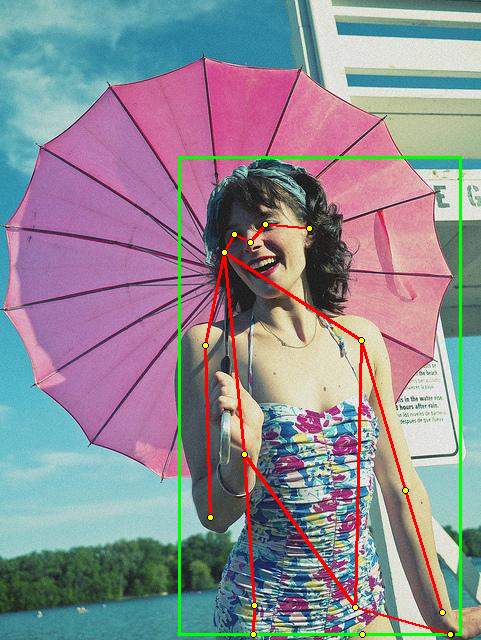
\includegraphics[width=\linewidth]{figures/demo_keypoints_overlay.png}
    \caption{\cmd{yolozu demo keypoints}}
  \end{subfigure}\hfill
  \begin{subfigure}[t]{0.32\linewidth}
    \centering
    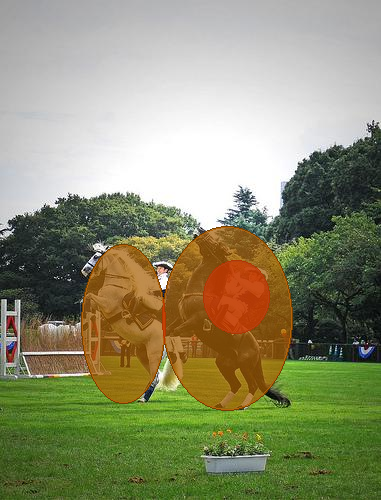
\includegraphics[width=\linewidth]{figures/demo_instance_seg_overlay.png}
    \caption{\cmd{yolozu demo instance-seg}}
  \end{subfigure}\hfill
  \begin{subfigure}[t]{0.32\linewidth}
    \centering
    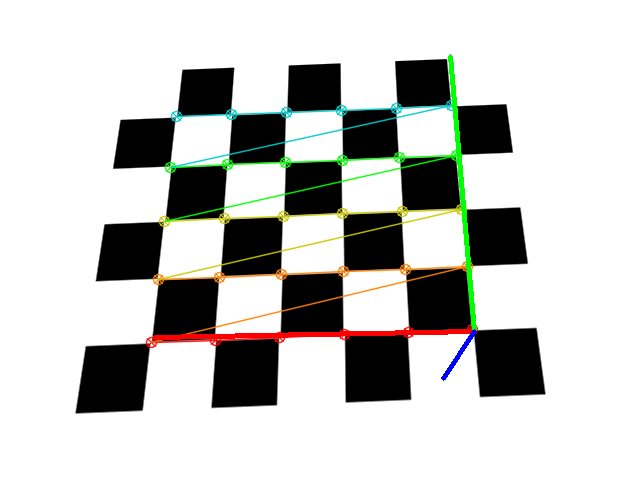
\includegraphics[width=\linewidth]{figures/demo_pose_overlay.png}
    \caption{\cmd{yolozu demo pose --backend aruco}}
  \end{subfigure}
  \caption{Real-image outputs from the keypoints, instance segmentation, and 6DoF pose demos. The tasks differ, but all stay aligned with the predictions interface contract mindset.}
\end{figure}

The corresponding commands are:
\begin{lstlisting}[language=bash]
python3 -m pip install -U 'yolozu[demo]'
yolozu demo keypoints
python3 scripts/download_coco_instances_tiny.py --out-root data/coco --split val2017 --num-images 8 --seed 0
yolozu demo instance-seg --background coco-instances --inference auto --num-images 1 --max-instances 8 --score-threshold 0.25
yolozu demo pose --backend aruco
\end{lstlisting}

To enable the COCO instances (polygon) background for the instance-seg demo without long flags:
\begin{lstlisting}[language=bash]
python3 scripts/download_coco_instances_tiny.py
yolozu demo instance-seg
\end{lstlisting}

To run a visible raw-versus-TTA comparison on a corrupted real COCO image:
\begin{lstlisting}[language=bash]
yolozu demo instance-seg-tta --run-dir reports/demo_instance_seg_tta
\end{lstlisting}

\noindent This writes \path{reports/demo_instance_seg_tta/selected/overlay_raw.png},
\path{reports/demo_instance_seg_tta/selected/overlay_tta.png}, and
\path{reports/demo_instance_seg_tta/instance_seg_tta_demo_report.json}.


\section{Source Checkout (Repository Path)}
If you are operating directly within the repository (e.g., utilizing the training stack or power-user scripts), follow this procedure:
\begin{lstlisting}[language=bash]
python3 -m pip install -r requirements-test.txt
python3 -m pip install -e .
python3 -m pytest -q
\end{lstlisting}

The repository-only smoke and fresh-install evidence harnesses require this checkout:
\begin{lstlisting}[language=bash]
bash scripts/smoke.sh
bash scripts/fresh_install_journey.sh --run-dir /tmp/yolozu_fresh_install
\end{lstlisting}
The fresh-install harness creates a new virtual environment, installs from public PyPI, and records
the resolved version, exact commands, exit codes, elapsed times, logs, and stable-lane reports.
Use a new run directory for each invocation.


\section{Recommended Deployment Flow}
The canonical deployment pipeline follows this progression:
\begin{quote}
PyTorch \(\to\) ONNX \(\to\) TensorRT
\end{quote}

On macOS, you can typically run CPU-bound tooling (validation, evaluation, and ONNX Runtime CPU export).
Treat MPS as available only when the local Torch runtime reports success for
\cmd{torch.backends.mps.is_available()}.
If that check is false, treat the machine as CPU-only for \yolozu{} purposes.
Python itself can still create the environment with \cmd{venv} and \cmd{pip}; when MPS does not come up, the usual blocker is the Torch wheel/runtime combination rather than Python environment creation. Miniforge/conda is therefore a fallback for some Apple Silicon hosts, not a hard requirement.
TensorRT execution is generally Linux/NVIDIA-centric.
TensorRT workflows are covered in the Real-Time vs. Batch Inference chapter. The canonical pipeline strictly follows PyTorch $\rightarrow$ ONNX $\rightarrow$ TensorRT and includes parity checks at each stage.

\begin{figure}[h]
\centering
\resizebox{\linewidth}{!}{%
\begin{tikzpicture}[
  node distance=8mm and 10mm,
  font=\small,
  box/.style={draw, rounded corners, align=left, inner sep=6pt},
  lane/.style={draw, rounded corners, inner sep=5pt, fill=gray!6},
  arrow/.style={-{Latex[length=2mm]}, thick},
  dashedarrow/.style={-{Latex[length=2mm]}, thick, dashed}
]

\node[box] (torch) {\textbf{PyTorch artifact}\\
train/checkpoint\\
\path{runs/<run_id>/checkpoints/*}};
\node[box, right=14mm of torch] (onnx) {\textbf{ONNX artifact}\\
\path{model.onnx}\\
\path{model.onnx.meta.json}};
\node[box, right=14mm of onnx] (trt) {\textbf{TensorRT artifact}\\
\path{engine.plan}\\
\path{engine.meta.json}};

\node[box, below=12mm of onnx] (export) {\textbf{Runtime adapter}\\
torch / onnxrt / opencv-dnn / trt};
\node[box, right=16mm of export] (pred) {\textbf{Prediction artifact}\\
\path{predictions.json}\\
schema-valid + relocatable\\
\cmd{meta.export_settings}};
\node[box, right=16mm of pred] (eval) {\textbf{Validation reports}\\
\path{eval_suite.json}\\
\path{metrics_report.json}};

\draw[arrow] (torch) -- (onnx);
\draw[arrow] (onnx) -- (trt);

\draw[dashedarrow] (torch) -- node[midway, left]{\scriptsize torch} (export);
\draw[dashedarrow] (onnx) -- node[midway, right]{\scriptsize onnxrt / opencv} (export);
\draw[dashedarrow] (trt) -- node[midway, right]{\scriptsize tensorrt} (export);

\draw[arrow] (export) -- (pred);
\draw[arrow] (pred) -- (eval);

\begin{pgfonlayer}{bg}
\node[lane, fit=(torch)(onnx)(trt), label=above:{\textbf{Artifacts}}] {};
\node[lane, fit=(export), label=below:{\textbf{Runtime}}] {};
\node[lane, fit=(pred)(eval), label=below:{\textbf{Validation}}] {};
\end{pgfonlayer}

\end{tikzpicture}
}
\caption{Recommended deployment flow, grouped by artifact creation, runtime adaptation, and validation evidence.}
\end{figure}
%
